\documentclass[runningheads]{llncs}

\usepackage[utf8x]{inputenc}
\usepackage[T1]{fontenc}


% Text organization
\usepackage{comment}
\usepackage{csquotes}
\usepackage{caption} % subfigures
\usepackage{subcaption}


\usepackage{amsmath}
\usepackage{amsfonts}
\usepackage{amssymb}
\usepackage{stmaryrd}
\SetSymbolFont{stmry}{bold}{U}{stmry}{m}{n}
\newcommand*{\qeda}{\hfill\ensuremath{\blacksquare}}%
\newcommand*{\qedb}{\hfill\ensuremath{\square}}%
\newtheorem{fact}{Fact}[section]
\usepackage{latexsym}
\usepackage{cmll}
\usepackage{xspace}

% graphics
\usepackage{mathdots}
\usepackage{nicematrix}
\setcounter{MaxMatrixCols}{20}
\usepackage{rotating}
\usepackage{tikz}
\usepackage{xcolor}
\definecolor{keywordcolor}{rgb}{0.7, 0.1, 0.1} % red
\definecolor{commentcolor}{rgb}{0.4, 0.4, 0.4} % grey
\definecolor{symbolcolor}{rgb}{0.0, 0.1, 0.6}  % blue
\definecolor{sortcolor}{rgb}{0.1, 0.5, 0.1}    % green
\definecolor{aawhite}{rgb}{0.97,0.97,0.97}
\definecolor{awhite}{rgb}{0.90,0.90,0.90}
\definecolor{lgreen}{rgb}{0.94,1.0,0.98}
\definecolor{dgreen}{rgb}{0.0,0.3,0.1}
\definecolor{sgreen}{rgb}{0.0,0.7,0.3}
\definecolor{lgreen}{rgb}{0.94,1.0,0.98}
\definecolor{bgreen}{rgb}{0.00,0.50,0.25}
\definecolor{dblue}{rgb}{0.0,0.1,0.6}
\definecolor{lorange}{rgb}{1, .85, .60}
\definecolor{lblue}{rgb}{.80, .90, .95}
\definecolor{mixed}{rgb}{0.0,0.3,0.3}
\definecolor{dred}{rgb}{0.6,0.2,0.0}
\definecolor{sred}{rgb}{0.7,0.2,0.0}
\definecolor{ddred}{rgb}{0.3,0.1,0.0}
\definecolor{turq}{rgb}{0.28,0.82,0.80}
\definecolor{lyellow}{rgb}{1.00,0.97,0.94}
\definecolor{mygreen}{rgb}{0,0.6,0}
\definecolor{mygray}{rgb}{0.5,0.5,0.5}
\definecolor{mymauve}{rgb}{0.58,0,0.82}
\definecolor{codegreen}{rgb}{0,0.6,0}
\definecolor{codegray}{rgb}{0.5,0.5,0.5}
\definecolor{codepurple}{rgb}{0.58,0,0.82}
\definecolor{backcolour}{rgb}{0.96,0.96,0.96}

\usepackage{graphicx}

\usepackage{hyperref}
\hypersetup{
    colorlinks=true,
    linkcolor=sred,
    filecolor=magenta,
    urlcolor=cyan,
    citecolor=sgreen,
    bookmarks=true,
}


% code
\usepackage{listings}
\def\lstlanguagefiles{lstlean.tex}
\lstset{language=lean}
\usepackage{float}
\floatstyle{boxed}
\restylefloat{table}
\restylefloat{figure}

%\usepackage{listings}
%\renewcommand{\verb}{\lstinline}
%% Yarel related definitions
%\input{yarel-lst.tex}
%\lstdefinestyle{yarel-style}{
%	backgroundcolor=\color{backcolour},
%	commentstyle=\color{codegreen},
%	keywordstyle=\color{magenta},
%	numberstyle=\tiny\color{codegray},
%	stringstyle=\color{codepurple},
%	%	basicstyle=\fontsize{9}{13}\selectfont\ttfamily,
%	basicstyle=\ttfamily\footnotesize,
%	breakatwhitespace=false,
%	breaklines=true,
%	captionpos=b,
%	keepspaces=true,
%	numbers=left,
%	numbersep=5pt,
%	showspaces=false,
%	showstringspaces=false,
%	showtabs=false,
%	tabsize=2
%}
%\lstset{
%	language={yarel},
%%	basicstyle=\fontsize{9}{13}\selectfont\ttfamily,
%	basicstyle=\small\ttfamily, % Global Code Style
%	captionpos=b, % Position of the Caption (t for top, b for bottom)
%	extendedchars=true, % Allows 256 instead of 128 ASCII characters
%	tabsize=2, % number of spaces indented when discovering a tab
%	columns=fixed, % make all characters equal width
%	keepspaces=true, % does not ignore spaces to fit width, convert tabs to spaces
%	showstringspaces=false, % lets spaces in strings appear as real spaces
%	breaklines=true, % wrap lines if they don't fit
%	frame=trbl, % draw a frame at the top, right, left and bottom of the listing
%	frameround=tttt, % make the frame round at all four corners
%	framesep=4pt, % quarter circle size of the round corners
%	numbers=left, % show line numbers at the left
%	numberstyle=\tiny\ttfamily, % style of the line numbers
%	commentstyle=\color{yarelGreen}, % style of comments
%	keywordstyle=\color{mymauve}, % style of keywords
%	%	stringstyle=\color{yarelBlue}, % style of strings
%	identifierstyle=\color{dblue},
%	stringstyle=\color{orange},
%	backgroundcolor=\color{gray!5},
%	mathescape=true,
%	sensitive=false, % keywords are not case-sensitive
%}
%\newcommand{\verby}[1]{\lstinline[language=yarel,style=yarel-style]+#1+}
%% JAVA related definitions
%\input{java-lst.tex}
%\lstdefinestyle{java-style}{
%	backgroundcolor=\color{backcolour},
%	commentstyle=\color{codegreen},
%	keywordstyle=\color{magenta},
%	numberstyle=\tiny\color{codegray},
%	stringstyle=\color{codepurple},
%	basicstyle=\fontsize{9}{13}\selectfont\ttfamily,
%%	basicstyle=\ttfamily\footnotesize,
%	breakatwhitespace=false,
%	breaklines=true,
%	captionpos=b,
%	keepspaces=true,
%	numbers=left,
%	numbersep=5pt,
%	showspaces=false,
%	showstringspaces=false,
%	showtabs=false,
%	tabsize=2
%}
%\lstset{
%	language={java},
%	morekeywords={cached,case,default,extension,false,import,JAVA,WORKFLOWSLOT,let,new,null,private,create,switch,this,true,reexport,around,if,then,else, def, val, var, private, class, static, return, as, instanceof, for, override, boolean},
%	morekeywords=[2]{filter, toList, last, head},
%	keywordstyle=[2]\color{eclipseOrange}\textit,
%	morekeywords=[3]{FAST, NORMAL, IN, PROVIDED},
%	keywordstyle=[3]\color{eclipseBlue}\textsl,
%	morekeywords=[4]{},          % <-- Your keywords here (w/ orange)
%	keywordstyle=[4]\color{eclipseOrange},
%	morecomment=[l]{//},
%	morecomment=[s]{/*}{*/},
%	morestring=[b]",
%}
%\newcommand{\verbj}[1]{\lstinline[language=java,style=java-style]+#1+}
%\newcommand{\vj}[1]{\lstinline[language=java,style=java-style]+#1+}
%%% lstlisting stop definitions


% macro
% \newcommand{\svdots}{\scriptscriptstyle \boldsymbol \vdots}
\newcommand{\perm}[1]{\scriptstyle \left\rmoustache #1 \right\rmoustache}
\newcommand{\bloch}[2]{\Block[draw=white,fill=lblue,line-width=.5mm,rounded-corners]{#1}{#2}} % https://en.wikipedia.org/wiki/Ernest_Bloch
\newcommand{\oloch}[2]{\Block[draw=white,fill=lorange,line-width=.5mm,rounded-corners]{#1}{#2}}
\newcommand{\conv}[1]{\overbracket[.5pt][1pt]{\underbracket[.5pt][1pt]{#1}}}

\newcommand{\NN}{\mathbb{N}}
\newcommand{\ZZ}{\mathbb{Z}}
\newcommand{\RR}{\mathbb{R}}

\newcommand{\floor}[1]{\left\lfloor #1 \right\rfloor}

\newcommand{\gl}{\text{\guillemotleft}}
\newcommand{\gr}{\text{\guillemotright}}


\newcommand{\ORPP}{\mathsf{ORPP}}
\newcommand{\rppf}{\mathsf{f}}
\newcommand{\rppg}{\mathsf{g}}
\newcommand{\rpph}{\mathsf{h}}
\newcommand{\rppId}{\mathsf{Id}}
\newcommand{\rppNe}{\mathsf{Ne}}
\newcommand{\rppSu}{\mathsf{Su}}
\newcommand{\rppPr}{\mathsf{Pr}}
\newcommand{\rppSw}{\mathsf{Sw}}
\newcommand{\rppCo}{\fatsemi}
\newcommand{\rppPa}{\Vert}
\newcommand{\rppIt}{\mathsf{It}}
\newcommand{\rppIta}{\mathsf{Ita}}
\newcommand{\rppItr}{\mathsf{Itr}}
\newcommand{\rppIf}{\mathsf{If}}
\newcommand{\rppinc}{\mathsf{inc}}
\newcommand{\rppdec}{\mathsf{dec}}
\newcommand{\rppmul}{\mathsf{mul}}
\newcommand{\rppsquare}{\mathsf{square}}
\newcommand{\rppless}{\mathsf{less}}
\newcommand{\rppcp}{\mathsf{cp}}
\newcommand{\rppcpi}{\mathsf{cp_{input}}}
\newcommand{\rpptr}{\mathsf{tr}}
\newcommand{\rppcu}{\mathsf{cu}}
\newcommand{\rppcui}{\mathsf{cu_{input}}}
\newcommand{\rppcustep}{\mathsf{cu_{step}}}
\newcommand{\rppdiv}{\mathsf{div}}
\newcommand{\rppdivstep}{\mathsf{div_{step}}}
\newcommand{\rppsqrt}{\mathsf{sqrt}}
\newcommand{\rppsqrtstep}{\mathsf{sqrt_{step}}}
\newcommand{\rpprewire}[1]{\lfloor #1 \rceil}
\newcommand{\rppmkpair}{\mathsf{mkpair}}
\newcommand{\rppmkpairi}{\mathsf{mkpair_{input}}}
\newcommand{\rppunpair}{\mathsf{unpair}}
\newcommand{\rppunpairi}{\mathsf{unpair_{input}}}
\newcommand{\rppunpairifwd}{\mathsf{unpair_{input, \rightarrow}}}
\newcommand{\rppprecstep}{\mathsf{prec_{step}}}
\newcommand{\rppprecfwd}{\mathsf{prec_{\rightarrow}}}
\newcommand{\rppprec}{\mathsf{prec}}
\newcommand{\rppconvert}{\mathsf{convert}}
\newcommand{\rppNu}{\mathsf{Nu}}
\newcommand{\rppZe}{\mathsf{Ze}}
\newcommand{\rppEz}{\mathsf{Ez}}
\newcommand{\rppbin}{\mathsf{bin}}


\newcommand{\prZero}{\mathtt{0}}
\newcommand{\prSucc}{\mathtt{S}}
\newcommand{\prPred}{\mathtt{P}}
\newcommand{\prProj}[2]{\mathtt{P}^{#1}_{#2}} % P^n_i
\newcommand{\prCom}[1]{\circ{[#1]}} % composition
\newcommand{\prPrec}{\mathtt{R}}
\newcommand{\pradd}{\mathtt{ADD}}
\newcommand{\prack}{\mathtt{ACK}}

% Macros
\newcommand{\RPP}{\textsf{RPP}\xspace}
\newcommand{\UPRF}{\textsf{UPRF}\xspace}
\newcommand{\PRF}{\textsf{PRF}\xspace}
\newcommand{\PR}{\textsf{PR}\xspace}
\newcommand{\CPP}{\textsf{C}\xspace}
\newcommand{\MATHLIB}{\textsf{mathlib}\xspace}
\newcommand{\LEAN}{\textsf{Lean}\xspace}
\newcommand{\LEANFour}{\textsf{Lean 4}\xspace}
\newcommand{\RPRF}{\textsf{R}\PRF\xspace} % reversible primitive
\newcommand{\JMF}{\textsf{RI}\xspace} % Jacopini Mentrasti
\newcommand{\Janus}{\textsf{Janus}\xspace}
\newcommand{\Matita}{\textsf{Matita}\xspace}
\newcommand{\SRL}{\textsf{SRL}\xspace}
\newcommand{\Nat}{\mathbb{N}}
\newcommand{\Int}{\mathbb{Z}}
\newcommand{\yb}{\textcolor{blue}{y}}
\newcommand{\yr}{\textcolor{red}{y}}


\begin{document}
%\title{A formal certification that Reversible Primitive Permutations are Primitive-recursive complete}
\title{Certifying algorithms and relevant properties of Reversible Primitive Permutations with \LEAN}
\titlerunning{Certifying \RPP properties with \LEAN}

\author{Giacomo Maletto\inst{1} \and
	    Luca Roversi\inst{2}\orcidID{0000-0002-1871-6109}}

\authorrunning{G. Maletto, L. Roversi}

\institute{
    Università degli Studi di Torino, Dipartimento di Matematica  -- Italy\\
	\email{giacomo.maletto@edu.unito.it}\\
	\and
	Università degli Studi di Torino, Dipartimento di Informatica -- Italy\\
	\email{luca.roversi@unito.it}}

\maketitle
\begin{abstract}
%TODO
\end{abstract}

%=====================
\section{Introduction}
\label{section:Introduction}
Studies focused on questions posed by Maxwell, regarding the sensibility of the principles which Thermodynamics is based on, recognized the fundamental role that Reversible Computation can play to that purpose.

Once identified, it has been apparent that Reversible Computation constitutes the context in which to frame relevant aspects in areas of Computer Science; they can span from reversible hardware design which can offer a greener foot-print, as compared to classical hardware, to unconventional computational models --- we think to quantum or bio-inspired ones, for example ---, passing through parallel computation and the synchronization issues that it rises, or debuggers that help tracing back to the origin of a bug, or the consistent transactions roll-back in data-base management systems, just to name some. The book \cite{perumalla2013chc} is a comprehensive introduction to the subject; the book \cite{DBLP:books/daglib/0025734}, focused on the low-level aspects of Reversible Computation, concerning the realization of reversible hardware, and
\cite{DBLP:series/eatcs/Morita17}, focused on how models of Reversible Computation like Reversible Turing Machines (RTM), and Reversible Cellular Automata (RCA) can be considered universal and how to prove that they enjoy such a property, can be considered complementary and integrate \cite{perumalla2013chc}.

This work focuses on the \emph{functional model} \RPP \cite{DBLP:journals/tcs/PaoliniPR20} of Reversible Computation.
\RPP stands for (the class of) Reversible Primitive Permutations, which can be seen as a possible reversible counterpart of \PRF, the class of Primitive Recursive functions \cite{rogers1967theory}.
We recall that \RPP, in analogy with \PRF, is defined as the smallest class built on some given basic reversible function,
and which is closed under suitable composition schemes.

The very functional nature of the elements in \RPP is at the base of reasonably accessible proofs of the following properties:
\begin{itemize}
\item \RPP is \PRF-complete, i.e. every function $ f $ in \PRF has a counterpart $ \hat{f} $ in \RPP that simulates $ f $ \cite{DBLP:journals/tcs/PaoliniPR20};

\item \RPP can be naturally extended to become Turing-complete \cite{Paolini2018NGC} by means of a composition scheme analogous to the one that extends \PRF to the Turing-complete class \PR of Partial Recursive functions;

\item According to \cite{MatosRC2020}, \RPP and the reversible programming language \SRL \cite{matos03tcs} are equivalent, so the fix-point problem is undecidable for \RPP as well \cite{2318_1734164MatosPaoliniRoversiTCSICTCS18}.
\end{itemize}

The motivation to write this work is to bring evidence that expressing Reversible Computation by means of recursively defined computational models, like the class \RPP, \emph{naturally} offers the possibility to certify the correctness, or other interesting properties, of reversible algorithms, by means of some proof-assistant.
We recall that proof-assistants supply an integrated environment to formalize data-types, to implement algorithms that work on those data-types, to formalize specifications of the implementations, and to prove in full detail that those implementation match their specifications, increasing their dependability.

%%%%%%%%%%%%%%%%%%%%%%%%%%%%
\paragraph{Contributions.}
Roughly, we show how to express \RPP and its evaluation mechanism inside the proof-assistant \LEAN \cite{Lean3}. On one side we are able to certify the correctness of every reversible function that we write in \RPP with respect to a given specification. On the other, we certify the correctness of the main result in \cite{DBLP:journals/tcs/PaoliniPR20} which states that \RPP is \PRF-complete. In more detail:
\begin{itemize}
    \item we give a strong guarantee that \RPP is \PRF-complete.
    Relying on existing proofs that the classes \PRF and \UPRF --- the class of \emph{Unary} Primitive recursive Functions ---, are equivalent, using the library \MATHLIB of the proof-assistant \LEAN, we prove that, for every function $ f $ of \UPRF, a function in \RPP exists that represents and simulates $ f $.
    Apart from fixing some small bugs, we provide a \PRF-completeness proof of \RPP \cite{DBLP:journals/tcs/PaoliniPR20} which is fully detailed, conceptually, and technically simpler;

    \item on one side the simplification is a consequence of the representation of \UPRF in \MATHLIB \LEAN library. On the other, and more remarkably,  the two following aspects characterize the simplifications:
    \begin{itemize}
        \item we introduce a finite reversible iteration scheme which is more primitive, but expressive enough to encode the finite reversible iteration schemes originally in \RPP, and \SRL;
        \item we completely rework and simplify the algorithm that implements Cantor Pairing \cite{Cantor1878,DBLP:journals/corr/Szudzik17} in \RPP \cite{DBLP:journals/tcs/PaoliniPR20}.
        We recall that Cantor Pairing is an isomorphism $ \mathbb{N}\times\mathbb{N} \simeq \mathbb{N} $. Inside the original proof of \PRF-completeness, Cantor Pairing works as a stack in order to correctly manage the computation of a recursive scheme of \UPRF by means of an element in \RPP. The \PRF-completeness that we develop in \LEAN does not rely on Cantor Pairing, but on an isomorphism $ \mathbb{N}\times\mathbb{N} \simeq \mathbb{N} $ in \MATHLIB \LEAN library.
    \end{itemize}

    \item we show that the \RPP function that we define to implement Cantor Pairing is one possible instance of a more general pattern that allows us to uniquely associate pairs of $ \mathbb{N}\times\mathbb{N}$ to a single element of $ \mathbb{N}$. This means that we are able to show further isomorphism $ \mathbb{N}\times\mathbb{N}\simeq \mathbb{N}$ in \RPP by just modifying a core of Cantor Pairing.
\end{itemize}

%---------------------
\paragraph{Related work.}
Works that relate algorithms implemented by means of a formalism that can express Reversible Computation seems not to abound. We are aware of \cite{paoliniTYPES2015}. By means of the proof-assistant \Matita \cite{Asperti2007}, it certifies that a denotational semantics for the imperative reversible programming language \Janus \cite[Section 8.3.3]{perumalla2013chc} is fully abstract with respect to the operational semantics.

An early proposal to express reversible computations in a functional formalism is \cite{jacopini89tcs}. It introduces the class \JMF of reversible functions which is as expressive as \PR. So, \JMF is stronger than \RPP, but we see \JMF as less abstract than \RPP for two reasons: (i) the primitive functions of \JMF depend on a given specific binary representation of natural numbers; (ii) unlike \RPP, which we can see as \PRF in a reversible setting, it is not evident to us that \JMF can be considered the natural extension of a total class analogous to \RPP.

%---------------------
\paragraph{Contents.}
This work illustrates the relevant parts of the BSc Thesis \cite{MalettoBSc2021} which comes with \cite{MalettoRPPLEAN2021}, a \LEAN project that certifies algorithms and properties of \RPP.
Section~\ref{section:Reversible Primitive Permutations} recalls the class \RPP by commenting on the main design aspects that characterize its definition inside \LEAN.
Section~\ref{section:RPP algorithms} defines and proves correct new reversible algorithms central to prove that \RPP is \PRF-complete.
Section~\ref{section:Unary Primitive Recursive Functions} recalls the main aspects of \UPRF, with particular attention to the computational behavior of its recursion scheme.
Section~\ref{section:The UPRF-completeness of RPP} illustrates the points that characterize the porting of the original proof that \RPP is \PRF-complete to \LEAN.
Section~\ref{section:Conclusion and developments} underlies further more general contribution of the work, a reason why we choose \LEAN,  and natural developments.

%=====================
\section{Reversible Primitive Permutations (\RPP) }
\label{section:Reversible Primitive Permutations}

\begin{figure}
    \centering
        \begin{lstlisting}
        inductive RPP : Type
        -- Base functions
        | Id (n : ℕ) : RPP -- Identity
        | Ne : RPP         -- Sign-change
        | Su : RPP         -- Successor
        | Pr : RPP         -- Predecessor
        | Sw : RPP         -- Transposition
        -- Inductively defined functions
        | Co (f g : RPP) : RPP   -- Parallel composition
        | Pa (f g : RPP) : RPP   -- Series composition
        | It (f : RPP) : RPP     -- Finite iteration
        | If (f g h : RPP) : RPP -- Selection
        infix `‖`  : 55 := Pa -- Notation for the Parallel composition
        infix `;;` : 50 := Co -- Notation for the Series composition
        \end{lstlisting}
    \caption{The class \RPP as a data-type \lstinline|RPP| in \LEAN.}
    \label{fig:RPP-LEAN}
\end{figure}

We use the data-type \lstinline|RPP| in Figure~\ref{fig:RPP-LEAN}, as defined in \LEAN, to recall from \cite{DBLP:journals/tcs/PaoliniPR20} that the class \RPP is the smallest class of functions
that contains five base functions, named as in the definition, and all the functions that we can generate by the composition schemes whose name is next to the corresponding clause in Figure~\ref{fig:RPP-LEAN}. For ease of use and readability the  last two lines in Figure~\ref{fig:RPP-LEAN} introduce infix notations for series and parallel compositions.

\begin{example}[A  term of type {\normalfont \lstinline|RPP|}]
\label{example:A first legal term of type RPP}
In \lstinline|RPP| we can write
\lstinline|(Id 1‖Sw);;(It Su)‖(Id 1);;(Id 1‖If Su (Id 1) Pr)| which we can also represent as a diagram whose inputs are the names to the left of the blocks, and outputs to the right:
\[
\begin{NiceMatrix}
x_0&\bloch{1-1}{\mbox{\lstinline|Id 1|}}&y_0&\bloch{2-1}{\mbox{\lstinline|It  Su|}}&w_0&\bloch{1-1}{\mbox{\lstinline|Id 1|}}&z_0
\\
x_1&\bloch{2-1}{\mbox{\lstinline|Sw|}}&y_1& &w_1&\bloch{2-1}{\mbox{\lstinline|If Su (Id 1) Pr|}}&z_1
\\
x_2&&y_2&\bloch{1-1}{\mbox{\lstinline|Id 1|}}&w_2&
&z_2
\end{NiceMatrix}
\enspace .
\]
The term we have just defined is a series composition of three parallel compositions.
We comment the structure of the first one, the others being similar: it is a parallel composition between a ``single wire'' \lstinline|Id 1| and the transposition \lstinline|Sw|.
\qeda
\end{example}

\begin{remark}[``Weak weakening'' of algorithms in {\normalfont \lstinline|RPP|}]
\label{remark:Weakening algorithms of RPP}
%We can certify that \lstinline|(f‖(Id m)) X = f X|, but not
%\lstinline|((Id m)‖f) X = f X|, for any $ \lstinline|X| $.
We typically drop \lstinline|Id m| if it is the last function of a parallel composition. For example, term and diagram in \textit{Example}~\ref{example:A first legal term of type RPP} become \lstinline|(Id 1‖Sw);;(It Su);;(Id 1‖If Su (Id 1) Pr)| and:
\[
\begin{NiceMatrix}
    x_0&\bloch{1-1}{\mbox{\lstinline|Id 1|}}&y_0&\bloch{2-1}{\mbox{\lstinline|It  Su|}}&w_0&\bloch{1-1}{\mbox{\lstinline|Id 1|}}&z_0
    \\
    x_1&\bloch{2-1}{\mbox{\lstinline|Sw|}}&y_1& &w_1&\bloch{2-1}{\mbox{\lstinline|If Su (Id 1) Pr|}}&z_1
    \\
    x_2&&y_2&&w_2&
    &z_2
\end{NiceMatrix}
\enspace .
\]
\textit{Remark}~\ref{remark:We keep the definition of ev simple} explains why.
\qeda
\end{remark}

\begin{figure}
\centering
\begin{lstlisting}
      def arity : RPP → ℕ
        | (Id n)     := n
        | Ne         := 1
        | Su         := 1
        | Pr         := 1
        | Sw         := 2
        | (f ‖ g)    := f.arity + g.arity
        | (f ;; g)   := max f.arity g.arity
        | (It f)     := 1 + f.arity
        | (If f g h) := 1 + max (max f.arity g.arity) h.arity
\end{lstlisting}
\caption{Arity of every \lstinline|f: RPP|.}
\label{fig:RPP-arity}
\end{figure}

The function in Figure~\ref{fig:RPP-arity} computes the arity of any \lstinline|f:RPP| from the structure of \lstinline|f|, once fixed the arities of the base functions.

\begin{figure}
    \begin{subfigure}{.5\textwidth}
        \centering
        $\begin{NiceMatrix}
            x_0&\bloch{1-1}{\mbox{\lstinline|Id 1|}}&y_0
            \\
            &\vdots&
            \\
            x_{n-1}&\bloch{1-1}{\mbox{\lstinline|Id 1|}}&y_{n-1}
        \end{NiceMatrix}$
        \caption{\lstinline|n| unary identities of \RPP in parallel.}
        \label{fig:Id 1 || .. || Id 1}
    \end{subfigure}
    \hfill
    \begin{subfigure}{.45\textwidth}
        \centering
        $ \begin{NiceMatrix}
            x_0&\bloch{3-1}{\mbox{\lstinline|Id n|}}&y_0
            \\
            \vdots&&\vdots
            \\
            x_{n-1}&&y_{n-1}
        \end{NiceMatrix} $
        \caption{Single \lstinline|n|-ary identity \lstinline|RPP|.}
        \label{fig:Id n}
    \end{subfigure}
    \caption{\lstinline|n|-ary identities are base functions of \lstinline|RPP|.}
    \label{fig:multiple-wires}
\end{figure}

Figure~\ref{fig:multiple-wires}, remarks that \lstinline|RPP| considers \lstinline|n|-ary identities \lstinline|Id n| as primitive; in original \RPP, \lstinline|Id n| is the parallel composition of \lstinline|n| unary identities.

\begin{figure}
\begin{lstlisting}
    def inv : RPP → RPP
      | (Id n)     := Id n -- self-dual
      | Ne         := Ne   -- self-dual
      | Su         := Pr
      | Pr         := Su
      | Sw         := Sw   -- self-dual
      | (f ‖ g)    := inv f ‖ inv g
      | (f ;; g)   := inv g ;; inv f
      | (It f)     := It (inv f)
      | (If f g h) := If (inv f) (inv g) (inv h)
    notation f `⁻¹` := inv f
\end{lstlisting}
\caption{Inverse \lstinline|inv f| of every \lstinline|f:RPP|.}
\label{fig:RPP-inv}
\end{figure}

For any given \lstinline|f:RPP|, the function \lstinline|inv| in Figure~\ref{fig:RPP-inv} builds an element with type \lstinline|RPP|. The definition of \lstinline|inv| let the successor \lstinline|Su| be inverse of the predecessor \lstinline|Pr| and let every other base function be self-dual.
Moreover, the function \lstinline|inv| distributes over finite iteration \lstinline|It|, selection \lstinline|If|, and parallel composition \lstinline|‖|, while it requires to exchange the order of the arguments before distributing over the series composition \lstinline|;;|. The last line with \lstinline|notation| suggests that \lstinline|f⁻¹| is the inverse of \lstinline|f|. We shall prove it once given the operational semantics of \lstinline|RPP|.

\begin{figure}
\begin{lstlisting}
def ev : RPP → list ℤ → list ℤ
| (Id n)     X                    := X
| Ne         (x :: X)             := -x :: X
| Su         (x :: X)             := (x + 1) :: X
| Pr         (x :: X)             := (x - 1) :: X
| Sw         (x :: y :: X)        := y :: x :: X
| (f ;; g)   X                    := ev g (ev f X)
| (f ‖ g)    X         := ev f (take f.arity X) ++ ev g (drop f.arity X)
| (It f)     (x :: X)             := x :: ((ev f)^[↓x] X)
| (If f g h) (0 :: X)             := 0 :: ev g X
| (If f g h) (((n : ℕ) + 1) :: X) := (n + 1) :: ev f X
| (If f g h) (-[1 + n] :: X)      := -[1 + n] :: ev h X
| _          X                    := X
notation `‹` f `›` := ev f -- ‹ \f ›
\end{lstlisting}
\caption{Operational semantics of elements in \lstinline|RPP|.}
\label{fig:RPP-ev}
\end{figure}

\paragraph{Operational semantics of {\normalfont \lstinline|RPP|}.}
The function \lstinline|ev| in Figure~\ref{fig:RPP-ev} interprets an element of \lstinline|RPP| as a function from a list of integers to a list of integers. Originally, in \cite{DBLP:journals/tcs/PaoliniPR20}, \RPP is a class of functions with type $ \ZZ^n \rightarrow \ZZ^n $. We use \lstinline|list ℤ| in place of tuples of \lstinline|ℤ| to exploit the rich \LEAN library of properties on lists to save quite a large amount of formalization work.

Let us give a look at the clauses in Figure~\ref{fig:RPP-ev}.
\lstinline|Id n| leaves the input list \lstinline|X| untouched.
\lstinline|Ne| negates the head of the list, \lstinline|Su| increments, and \lstinline|Su| decrements it.
\lstinline|Sw| is the transposition that switches the first two elements of its argument.
The series composition \lstinline|f;;g| first applies \lstinline|f| and then
\lstinline|g|.
The parallel composition \lstinline|f‖g| splits \lstinline|X| into two parts. The ``topmost'' one \lstinline|take f.arity X| has as many elements as the arity of \lstinline|f|; the ``lowermost'' one \lstinline|drop f.arity X| contains the part of \lstinline|X| that can supply the arguments to \lstinline|g|. Finally, it concatenates the two resulting lists by the append \lstinline|++|. The finite iteration
\lstinline|It f| iterates \lstinline|f| as many times as the value of the head \lstinline|x| of the argument, if \lstinline|x| contains a non negative value; otherwise it is the identity on the whole \lstinline|x::X|. This behavior is the meaning of \lstinline|(ev f)^[↓x]|.
The selection \lstinline|If f g h| chooses one among \lstinline|f|, \lstinline|g|, and \lstinline|h|, depending on the argument head \lstinline|x|: it is \lstinline|g| with \lstinline|x = 0|, it is \lstinline|f| with \lstinline|x > 0|, and \lstinline|h| with \lstinline|x < 0|.
The last line of Figure~\ref{fig:RPP-ev} sets a handy notation for \lstinline|ev|.

\begin{remark}[We keep the definition of {\normalfont \lstinline|ev|} simple]
\label{remark:We keep the definition of ev simple}
We can prove that the definition of \lstinline|ev| allows us to apply any \lstinline|f:RPP| to any \lstinline|X:list ℤ|.
If \lstinline|X.length >= f.arity|, i.e. \lstinline|X| supplies enough arguments, then \lstinline|f| operates on the first elements of \lstinline|X| according to its arity. This justifies \textit{Remark}~\ref{remark:Weakening algorithms of RPP}. If \lstinline|X.length < f.arity|, i.e. \lstinline|X| has not enough elements, \lstinline|f X| has an unspecified behavior. This might sound odd, but it simplifies the proofs of must-have properties of \lstinline|RPP|.
%This is possible because we can prove:
%\begin{lstlisting}
%    lemma ev_length (f: RPP) (X: list ℤ): (‹f› X).length = X.length
%    theorem ev_split (f: RPP) (X: list ℤ):
%    ‹f› X = ‹f›(take f.arity X) ++ drop f.arity X .
%\end{lstlisting}
%\lstinline|lemma ev_length| says that \lstinline|RPP| functions preserve the argument length.
%One of the most complex property to prove correct, i.e. \lstinline|theorem ev_split|, says that we can apply any \lstinline|‹f›| to \emph{any} \lstinline|X| with at least as many elements as \lstinline|arity f|.
\qeda
\end{remark}

%======================
\subsection{The functions {\normalfont \lstinline|inv f|} and {\normalfont \lstinline|f|} are each other inverse}
Once defined \lstinline|inv| in Figure~\ref{fig:RPP-inv} and \lstinline|ev| in Figure~\ref{fig:RPP-ev} we can prove both:
\begin{lstlisting}
    theorem inv_co_l (f : RPP) (X : list ℤ) : ‹f ;; f⁻¹› X = X
    theorem inv_co_r (f : RPP) (X : list ℤ) : ‹f⁻¹ ;; f› X = X .
\end{lstlisting}
We start by focusing on the main details to prove \lstinline|theorem inv_co_l| in \LEAN. The proof proceeds by (structural) induction on \lstinline|f|, which generates 9 cases, one for each clause that defines \lstinline|RPP|. One can go through the majority of them smoothly.
Some comments about the more challenging cases follow.

\paragraph{Series composition.} Let \lstinline|f| be \lstinline|Co|. The step-wise proof of \lstinline|inv_co_l| is:
\begin{lstlisting}
‹(f;;g);;(f;;g)⁻¹› X
     = ‹f⁻¹›(‹g⁻¹›(‹g›(‹f› X))) -- by definition
     = ‹f⁻¹›(‹g;;g⁻¹ (‹f› X))   -- by a general ind. hyp.
 (!) = ‹f⁻¹›(‹f› X)             -- by definition
     = ‹f;;f⁻¹› X               -- by a general ind. hyp.
     = X ,
\end{lstlisting}
where the equivalence \lstinline|(!)| holds thanks to the right inductive hypothesis on the behavior of \lstinline|g;;g⁻¹| that \emph{must} be
\lstinline|∀ (X : list ℤ), ‹g;;g⁻¹› X = X|.
\qedb

\paragraph{Parallel composition.} Let \lstinline|f| be \lstinline|Pa|. The step-wise proof of \lstinline|inv_co_l| is:
\begin{lstlisting}
‹f‖g;;(f‖g)⁻¹› X              -- by definition
     = ‹f‖g;;f⁻¹‖g⁻¹› X       -- not obvious
 (!) = ‹(f;;f⁻¹)‖(g;;g⁻¹)› X  -- by definition
     = ‹f;;f⁻¹›(take f.arity X)++‹g;;g⁻¹›(drop f.arity X) -- by ind. hyp.
     = take f.arity X ++ drop f.arity X -- property of ++ (append)
     = X ,
\end{lstlisting}
where the equivalence \lstinline|(!)| holds because we can prove both:
\begin{lstlisting}
lemma pa_co_pa (f f' g g' : RPP) (X : list ℤ) :
  f.arity = f'.arity → ‹f‖g ;; f'‖g'› X = ‹(f;;f') ‖ (g;;g')› X ,
lemma arity_inv (f : RPP) : f⁻¹.arity = f.arity .
\end{lstlisting}
Proving \lstinline|lemma arity_inv|, i.e. that the arity of a function does not change if we invert it, assures that we can prove \lstinline|lemma pa_co_pa|, i.e. that series and parallel compositions smoothly distribute reciprocally.
\qedb

\paragraph{Iteration.} Let \lstinline|f| be \lstinline|It|.
In this case, the most complex goal to prove is \lstinline|‹It f;;It f⁻¹› x::X = x::X| which reduces to \lstinline|‹f⁻¹›^[↓x] (‹f›^[↓x] X') = X'|, where, we recall, the notation \lstinline|‹f›^[↓x]| means ``\lstinline|‹f›| applied \lstinline|x| times, if \lstinline|x| is positive''. Luckily this last statement is both formalized as \lstinline|function.left_inverse (g^[n]) (f^[n])|, and proven in the library \MATHLIB of \LEAN, where \lstinline|function.left_inverse| is the proposition \lstinline|∀ (g: β → α) (f: α → β) (x: α), g(f x) = x : Prop|, with \lstinline|α|, and \lstinline|β| generic types.
\qedb

\vspace{\baselineskip}
To conclude, let us see how the proof of \lstinline|inv_co_r| works. It does not copy-cat the one of \lstinline|inv_co_l|. It relies on proving:
\begin{lstlisting}
   lemma inv_involute (f : RPP) : (f⁻¹)⁻¹ = f ,
\end{lstlisting}
\noindent
which says that applying \lstinline|inv| twice is the identity, and on using \lstinline|inv_co_l|:
\begin{lstlisting}
    ‹f⁻¹ ;; f› X = X -- which, by inv_involute, is equivalent to
    ‹f⁻¹ ;; (f⁻¹)⁻¹› X = X -- which holds because it is an instance of (inv_co_l f⁻¹) .
\end{lstlisting}

\begin{remark}[On our simplifying choices on {\normalfont \lstinline|ev|}]
\label{remark:On our simplifying choices on ev}
A less general, but semantically more appropriate versions of  \lstinline|inv_co_l| and \lstinline|inv_co_r| could be:
\begin{lstlisting}
    theorem inv_co_l (f : RPP) (X : list ℤ) :
                f.arity ≤ X.length → ‹f ;; f⁻¹› X = X
    theorem inv_co_r (f : RPP) (X : list ℤ) :
                f.arity ≤ X.length → ‹f⁻¹ ;; f› X = X
\end{lstlisting}
because, recalling \textit{Remark}~\ref{remark:We keep the definition of ev simple}, \lstinline|f X| makes sense when \lstinline|f.arity ≤ X.length|.
Fortunately, the way we defined \lstinline|RPP| allows us to state \lstinline|inv_co_l| or \lstinline|inv_co_r| in full generality
with no reference to \lstinline|f.arity ≤ X.length|.
\qeda
\end{remark}

%======================
\subsection{How {\normalfont \lstinline|RPP|} differs from original {\normalfont \RPP}}
The definition of \lstinline|RPP| of \LEAN is really very close to the original \lstinline|RPP|, but not identical. The goal is to simplify the overall task of formalization and certification. The brief list of changes follows.
\begin{itemize}
    \item As already outlined, \lstinline|It| and \lstinline|If| use the head of the input list to iterate or choose, because \LEAN pattern matching makes it obvious to take the head of a list. On the contrary, both iteration and selection of \RPP were driven by the value of the last element in the input tuple.

    \item \lstinline|Id n|, for any \lstinline|n:ℕ|, is primitive in \lstinline|RPP| and derived in \RPP. In some cases it is useful to have \lstinline|Id 0| available.

    \item Using \lstinline|list ℤ → list ℤ| as the domain of the function that interpets any given element \lstinline|f:RPP| avoids to let the type of \lstinline|f:RPP| depend on the arity of \lstinline|f|. To know the arity of \lstinline|f| it is enough to invoke \lstinline|arity f|. Finally, we observe that getting rid of a dependent type like, say, \lstinline|RPP n|, allows us to escape situations in which we would need to prove that \lstinline|RPP (n+1)| and \lstinline|RPP (1+n)| are the same type.

    \item The finite iterator \lstinline|It f (x::t): list ℤ| subsumes the finite iterators \lstinline|ItR| in \RPP, and \lstinline|for| in \SRL.

    We recall that \lstinline|ItR f (x₀,x₁,...,xₙ₋₂,x)| evalutes to \lstinline|f(f(...f(x₀,x₁,...,xₙ₋₂)...))| with $ \mid\!\!\mbox{\lstinline|x|}\!\!\mid $ occurrences of \lstinline|f|.
    Instead, \lstinline|for(f) x|\footnote{In fact, the syntax would be ``\lstinline|for x (f)|''. Our choice simplifies the translation \eqref{align:It for}.} evaluates to \lstinline|f(f(...f(x₀,x₁,...,xₙ₋₂)...))| with \lstinline|x| occurrences of \lstinline|f|, if \lstinline|x > 0|; it evaluates to \lstinline|f⁻¹(f⁻¹(...f⁻¹(x₀,x₁,...,xₙ₋₂)...))| with \lstinline|-x| occurrences of \lstinline|f⁻¹|, if \lstinline|x < 0|; it behaves like the identity if \lstinline|x = 0|.

    We can define both \lstinline|ItR| and \lstinline|for| in terms of \lstinline|It|:
    \begin{align}
    \label{align:It ItR}
        \mbox{\lstinline|ItR f|}
        & =
        \mbox{\lstinline|(It f);;Ne;;(It f);;Ne|} \\
    \label{align:It for}
        \mbox{\lstinline|for(f)|}
        & =
        \mbox{\lstinline|(It f);;Ne;;(It f⁻¹);;Ne|}
    \end{align}
    \begin{example}[How does \eqref{align:It ItR} work?]
    \label{example:How align:It ItR works}
    Whenever \lstinline|x > 0|, the leftmost \lstinline|It f| in \eqref{align:It ItR} iterates \lstinline|f|, while the rightmost one does nothing because \lstinline|Ne| in the middle negates \lstinline|x|.
    On the contrary, if \lstinline|x < 0|, the leftmost \lstinline|It f| does nothing and the iteration is performed by the rightmost iteration, because \lstinline|Ne| in the middle negates \lstinline|x|. In both cases, the last \lstinline|Ne| restores \lstinline|x| to its initial sign. But this is the behavior of \lstinline|ItR|, as we wanted. \qeda
    \end{example}

    Last, but not least, it's much easier to convince \LEAN that \lstinline|It| terminates, than it is for \lstinline|ItR| or \lstinline|for|.
\end{itemize}

%=====================
\section{{\normalfont \lstinline|RPP|} algorithms central to our proofs}
\label{section:RPP algorithms}

%    Comincio col dire che cp è una biezione N^2 -> N con inversa cu etc, che voglio esprimere dentro RPP.
%Osservo che è facile fare una funzione cp_in : (x,y,0) |-> (x,y,cp(x,y)), ma invece vorrei una funzione cp : (x,y) |-> (cp(x,y),0), che si sbarazza dell'input. L'obiettivo è quindi trovare una funzione che sia del tipo cu_in : (cp(x,y),0,0) |-> (cp(x,y),x,y) cosicché possiamo sbarazzarci dell'input facendone l'inversa.
%La formulazione "algebrica"/"analitica" di cu non è facilmente implementabile in RPP.
%Osserviamo invece che dato (x,y), cp(x,y) non è altro che il numero di passi da seguire in questo percorso per arrivare alla casella (x,y) a partire da (0,0). Allora per ottenere (x,y) a partire da cp(x,y) basta ragionare al contrario: partiamo da (0,0) e iteriamo cp(x,y) volte step, finendo alla fine in (x,y).
%(*) La difficoltà nel definire step sta nel fatto che la condizione è sulla variabile y, che allo stesso tempo è modificata nel calcolo. Questo va contro la definizione di condizionale di RPP. Il seguente algoritmo (step_[Su;;Sw]) riesce ad evitare questo problema "rigirando le variabili in modo furbo" (l'unico modo che ho trovato di descrivere questa cosa è come nella tesi: "We get around this limitation by using an ancillary variable initially set to 0, which assumes value 1 or 0 depending on whether y > 0 or y = 0, and is then set back to 0 using a variable that we know is positive or equal to zero depending on the case considered.").
%Avendo definito cp : (x,y) |-> (cp(x,y),0) abbiamo gratis l'inversa cu : (cp(x,y),0) |-> (x,y)
%
%L'unica cosa nuova è il punto (*), gli altri sono praticamente un riordinamento di quanto c'è già scritto.
%Scrivere le cose in questo modo significa esprimere tutto in termini di cp(x,y) anziché usare una variabile "n" e calcolare cu_1(n), cu_2(n).
%Inoltre renderebbe più chiaro come mai è stato difficile definire cp. Dimmi cosa ne pensi di questo approccio.
%

\begin{figure}
\begin{subfigure}{.225\textwidth}
\centering
$\begin{NiceMatrix}
    n & \bloch{2-1}{\mbox{\lstinline|It Su|}} & n     \\
    x &                      & x + n \\
 \end{NiceMatrix}$
\caption{Increment \lstinline|inc|}
\label{sfig:inc}
\end{subfigure}
\hfill
\begin{subfigure}{.225\textwidth}
\centering
$ \begin{NiceMatrix}
    n & \bloch{2-1}{\mbox{\lstinline|It Pr|}} & n     \\
    x &                      & x - n \\
  \end{NiceMatrix} $
\caption{Decrement \lstinline|dec|}
\label{sfig:dec}
\end{subfigure}
\hfill
\begin{subfigure}{.325\textwidth}
\centering
$ \begin{NiceMatrix}
    n & \bloch{3-1}{\mbox{\lstinline|It inc|}} & n             \\
    m &                     & m             \\
    x &                     & x + n \cdot m \\
  \end{NiceMatrix} $
\caption{Multiplication \lstinline|mul|}
\label{sfig:mul}
\end{subfigure}
\\
\begin{subfigure}{.6\textwidth}
\centering
$\begin{NiceMatrix}
    n &  \bloch{1-1}{\mbox{\lstinline|Id 1|}}  & n & \bloch{2-1}{\mbox{\lstinline|inc|}} & n & \bloch{3-1}{\mbox{\lstinline|mul|}} & n             & \bloch{2-1}{\mbox{\lstinline|dec|}} & n             & \bloch{1-1}{\mbox{\lstinline|Id 1|}}   & n
    \\
    x & \bloch{2-1}{\mbox{\lstinline|Sw|}} & 0 &   & n &                      & n             &                      & 0             & \bloch{2-1}{\mbox{\lstinline|Sw|}} & x + n \cdot n
    \\
    0 &                     & x &   & x &                      & x + n \cdot n &   \      & x + n \cdot n &                     & 0
\end{NiceMatrix}$
\caption{\lstinline|square|}
\label{fig:square}
\end{subfigure}
\hfill
\begin{subfigure}{.325\textwidth}
    \centering
    $\begin{NiceMatrix}
        x_0 & \bloch{6-1}{\rpprewire{i_0, \ldots, i_n}} & x_{i_0} \\
      \cdot &                                & \vdots  \\
      \cdot &                                & x_{i_n} \\
      \cdot &                                & x_{j_1} \\
      \cdot &                                & \vdots  \\
        x_m &                                & x_{j_{m-n}}
    \end{NiceMatrix}$
    \caption{Rewiring $ \rpprewire{i_0 \ldots i_n} $}
    \label{fig:rewiring}
\end{subfigure}
\caption{Some useful functions of \lstinline|RPP|}
\label{fig:standard functions}
\end{figure}

Figure~\ref{fig:standard functions} recalls definition and behavior of some \lstinline|RPP| functions already in \cite{DBLP:journals/tcs/PaoliniPR20}. It is worth commenting $ \rpprewire{i_0 \ldots i_n} $  Rewiring. Let $\{ i_0, \dots, i_n \} \subseteq \{ 0, \dots, m \}$; let $\{ j_1, \dots, j_{m-n} \}$ be $\{ 0, \dots, m \} \setminus \{ i_0, \dots, i_n \}$, i.e. the set of remaining indices, ordered such that $j_k < j_{k+1}$.
By definition, $\rpprewire{i_0, \dots, i_n} (x_0, \dots, x_m) = (x_{i_0}, \dots, x_{i_n},$ $x_{j_1}, \dots, x_{j_{m-n}})$, i.e. rewiring brings every input with index in $ \{ i_0, \dots, i_n \} $ before all the remaining inputs, by preserving order.

\begin{figure}
%    \centering
    \scalebox{.82}{
        $\begin{NiceMatrix}
            & a_0 &\bloch{1-1}{\mbox{\lstinline|Id 1|}}& b_0 & \bloch{3-1}{\rpprewire{2,0,1}} & c_0 & \bloch{3-1}{\mbox{\lstinline|If(Su‖Pr)[_](Id 1)|}}& d_0 & \bloch{2-1}{
                 \mbox{\lstinline|Sw|}
%                \rppSw
            } & e_0 & \bloch{2-1}{
                \mbox{\lstinline|If(Pr)(Id 1)(Id 1)|}
%                \rppIf[\boldsymbol{\rppPr}, \rppId_1, \rppId_1]
                } & f_0 &\bloch{1-1}{\mbox{\lstinline|Id 1|}}& g_0
            \\
            & a_1 & \bloch{2-1}{
                \mbox{\lstinline|If(Su)(Id 1)(Id 1)|}
%                \rppIf[\boldsymbol{\rppSu}, \rppId_1, \rppId_1]
            } & b_1 &&c_1&& d_1 & & e_1     &&f_1     & \bloch{2-1}{
                \mbox{\lstinline|Sw|}
%            \rppSw
        } & g_1
            \\
            & a_2&&b_2&&c_2&& d_2 && e_2 && f_2 && g_2
        \end{NiceMatrix}$
       }
    \caption{Algorithm scheme \lstinline|step[_]|. The algorithm we can obtain from it depends on how we fill the hole \lstinline|[_]|.}
    \label{fig:function scheme step}
\end{figure}

Figure~\ref{fig:function scheme step} identifies the new scheme of algorithm \lstinline|step[_]|. Depending on how we fill the hole \lstinline|[_]|, we obtain step functions that, once iterated draw paths into $ \NN^2 $. The names $ a_0, \ldots, b_0, \ldots $ are just place holders, currently.

\begin{figure}
\begin{subfigure}{.225\textwidth}
\centering
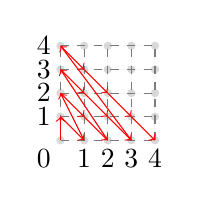
\begin{tikzpicture}[scale=0.3]
    % grid
    \draw[dashed,fill=gray,opacity=.5]  (0,0) grid (4,4);
    % labels
    \foreach \x in {1,...,4} { \node [anchor=north] at (\x,0) {\x}; }
    \foreach \y in {1,...,4} { \node [anchor=east] at (0,\y) {\y}; }
    \node [anchor=north east] at (0,0) {0};
    % vertices
    \foreach \x in {0,...,4} {
        \foreach \y in {0,...,4} {
            \node at (\x,\y) [circle,inner sep=0pt,minimum size=3pt,fill=gray,opacity=.3] {};
        }
    }
    % path
    \draw [->,red] (0,0) -- (0,1);
    \draw [->,red] (0,1) -- (1,0);
    \draw [->,red] (1,0) -- (0,2);
    \draw [->,red] (0,2) -- (1,1);
    \draw [->,red] (1,1) -- (2,0);
    \draw [->,red] (2,0) -- (0,3);
    \draw [->,red] (0,3) -- (1,2);
    \draw [->,red] (1,2) -- (2,1);
    \draw [->,red] (2,1) -- (3,0);
    \draw [->,red] (3,0) -- (0,4);
    \draw [->,red] (0,4) -- (1,3);
    \draw [->,red] (1,3) -- (2,2);
    \draw [->,red] (2,2) -- (3,1);
    \draw [->,red] (3,1) -- (4,0);
\end{tikzpicture}
\caption{Cantor.}
\label{sfig:cantor as a path}
\end{subfigure}
\hfill
\begin{subfigure}{.225\textwidth}
\centering
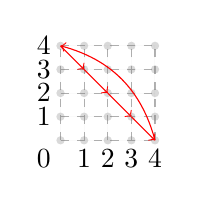
\begin{tikzpicture}[scale=0.3]
    % grid
    \draw[dashed,fill=gray,opacity=.3]  (0,0) grid (4,4);
    % labels
    \foreach \x in {1,...,4} { \node [anchor=north] at (\x,0) {\x}; }
    \foreach \y in {1,...,4} { \node [anchor=east] at (0,\y) {\y}; }
    \node [anchor=north east] at (0,0) {0};
    % vertices
    \foreach \x in {0,...,4} {
        \foreach \y in {0,...,4} {
            \node at (\x,\y) [circle,inner sep=0pt,minimum size=3pt,fill=gray,opacity=.3] {};
        }
    }
    % path
\draw [->,red] (4,0) to [bend right=30] (0,4);
\draw [->,red] (0,4) -- (1,3);
\draw [->,red] (1,3) -- (2,2);
\draw [->,red] (2,2) -- (3,1);
\draw [->,red] (3,1) -- (4,0);
\end{tikzpicture}
\caption{Quot./Rem.}
\label{sfig:Quot./Rem.}
\end{subfigure}
\hfill
\begin{subfigure}{.225\textwidth}
\centering
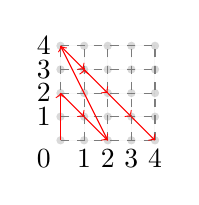
\begin{tikzpicture}[scale=0.3]
    % grid
    \draw[dashed,fill=gray,opacity=.5]  (0,0) grid (4,4);
    % labels
    \foreach \x in {1,...,4} { \node [anchor=north] at (\x,0) {\x}; }
    \foreach \y in {1,...,4} { \node [anchor=east] at (0,\y) {\y}; }
    \node [anchor=north east] at (0,0) {0};
    % vertices
    \foreach \x in {0,...,4} {
        \foreach \y in {0,...,4} {
            \node at (\x,\y) [circle,inner sep=0pt,minimum size=3pt,fill=gray,opacity=.3] {};
        }
    }
    % path
\draw [->,red] (0,0) -- (0,2);
\draw [->,red] (0,2) -- (1,1);
\draw [->,red] (1,1) -- (2,0);
\draw [->,red] (2,0) -- (0,4);
\draw [->,red] (0,4) -- (1,3);
\draw [->,red] (1,3) -- (1,3);
\draw [->,red] (1,3) -- (2,2);
\draw [->,red] (2,2) -- (3,1);
\draw [->,red] (3,1) -- (4,0);
\end{tikzpicture}
\caption{Square root.}
\label{sfig:Square root}
\end{subfigure}
\hfill
    \begin{subfigure}{.225\textwidth}
    \centering
    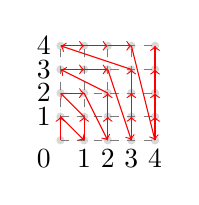
\begin{tikzpicture}[scale=0.3]
        % grid
        \draw[dashed,fill=gray,opacity=.5]  (0,0) grid (4,4);
        % labels
        \foreach \x in {1,...,4} { \node [anchor=north] at (\x,0) {\x}; }
        \foreach \y in {1,...,4} { \node [anchor=east] at (0,\y) {\y}; }
        \node [anchor=north east] at (0,0) {0};
        % vertices
        \foreach \x in {0,...,4} {
            \foreach \y in {0,...,4} {
                \node at (\x,\y) [circle,inner sep=0pt,minimum size=3pt,fill=gray,opacity=.3] {};
            }
        }
        % path
        \draw [->,red] (0,0) -- (0,1);
        \draw [->,red] (0,1) -- (1,0);
        \draw [->,red] (1,0) -- (1,1);
        \draw [->,red] (1,1) -- (0,2);
        \draw [->,red] (0,2) -- (1,2);
        \draw [->,red] (1,2) -- (2,0);
        \draw [->,red] (2,0) -- (2,1);
        \draw [->,red] (2,1) -- (2,2);
        \draw [->,red] (2,2) -- (0,3);
        \draw [->,red] (0,3) -- (1,3);
        \draw [->,red] (1,3) -- (2,3);
        \draw [->,red] (2,3) -- (3,0);
        \draw [->,red] (3,0) -- (3,1);
        \draw [->,red] (3,1) -- (3,2);
        \draw [->,red] (3,2) -- (3,3);
        \draw [->,red] (3,3) -- (0,4);
        \draw [->,red] (0,4) -- (1,4);
        \draw [->,red] (1,4) -- (2,4);
        \draw [->,red] (2,4) -- (3,4);
        \draw [->,red] (3,4) -- (4,0);
        \draw [->,red] (4,0) -- (4,1);
        \draw [->,red] (4,1) -- (4,2);
        \draw [->,red] (4,2) -- (4,3);
        \draw [->,red] (4,3) -- (4,4);
    \end{tikzpicture}
    \caption{Iso. $ \NN^2\simeq\NN $. }
    \label{sfig:4}
\end{subfigure}
\caption{Paths in a two dimensional space that generate algorithms in \lstinline|RPP|.}
\label{fig:functions as paths}
\end{figure}

On top of the functions in Figures~\ref{fig:standard functions}, and~\ref{fig:function scheme step} we build the Cantor Pairing/Un-pairing, quotient and reminder of integer division, and integer approximation of Square root. The point is to make the correct instance of \lstinline|step[_]| in order to visit $ \NN^2 $ with the paths in Figures~\ref{sfig:cantor as a path}, \ref{sfig:Quot./Rem.}, and~\ref{sfig:Square root}, respectively.

\paragraph{Cantor (Un-)Pairing}. The standard definition of Cantor Pairing $\rppcp : \NN^2 \to \NN$ and Un-pairing $\rppcu : \NN \to \NN^2$, two bijections one inverse of the other, is:
\begin{align}
\label{align: cp analitically}
\rppcp(x,y) & = \sum_{i=1}^{x+y}i + x = \frac{(x + y)(x + y + 1)}{2} + x
\\
\label{align: cu analitically}
\rppcu(n)  & = \left( n - \frac{i(1+i)}{2}, \frac{i(3+i)}{2} - n \right)
\enspace ,
\end{align}
where $i = \left\lfloor \frac{\sqrt{8n + 1} - 1}{2} \right\rfloor $.

\begin{figure}
\begin{subfigure}{.975\textwidth}
    \centering
\scalebox{.82}{
    $\begin{NiceMatrix}
        x &\bloch{2-1}{\mbox{\lstinline|inc|}}&x&\bloch{1-1}{\mbox{\lstinline|Id 1|}}&x&\bloch{1-1}{\mbox{\lstinline|Id 1|}}&\bloch{2-1}{\mbox{\lstinline|dec|}}&x& \bloch{4-1}{\rpprewire{0,3,1}} &\bloch{2-1}{\mbox{\lstinline|inc|}} &\bloch{1-1}{\mbox{\lstinline|Id 1|}} & x
        \\
        y && x + y & \bloch{3-1}{
            \mbox{\lstinline|It(Su;;inc)|}
            %            \rppIt[\rppSu \rppCo \rppinc]
        } & x + y& \bloch{2-1}{\mbox{\lstinline|dec|}} && y&&& \bloch{2-1}{\mbox{\lstinline|Sw|}} & y
        \\
        0 &                      & 0     &                     & x + y                &                      &                      & 0                    &                      &                      &                     & \sum_{i=1}^{x + y} i + x
        \\
        0 &                      & 0     &                     & \sum_{i=1}^{x + y} i &                      &                      & \sum_{i=1}^{x + y} i &                      &                      &                     & 0
    \end{NiceMatrix}$
}
    \caption{Function \lstinline|cp_in|}
    \label{sfig:cp input}
\end{subfigure}
\\
\begin{subfigure}{.975\textwidth}
\centering
\scalebox{.72}{
    $\begin{NiceMatrix}
        & x &\bloch{1-1}{\mbox{\lstinline|Id 1|}}& x & \bloch{3-1}{\rpprewire{2,0,1}} & 1 & \bloch{3-1}{
            \mbox{\lstinline|If(Su‖Pr)(Su;;Sw)(Id 1)|}
%            \rppIf[\boldsymbol{\rppSu \rppPa \rppPr}, \mbox{\lstinline|Su;;Sw|}, \ \rppId_1]
        } & 1     & \bloch{2-1}{
        \mbox{\lstinline|Sw|}
%        \rppSw
        } & x + 1 & \bloch{2-1}{
        \mbox{\lstinline|If(Pr)(Id 1)(Id 1)|}
%        \rppIf[\boldsymbol{\rppPr}, \rppId_1, \rppId_1]
        } & x + 1 &\bloch{1-1}{\mbox{\lstinline|Id 1|}} & x + 1 \\
        & \yb & \bloch{2-1}{
        \mbox{\lstinline|If(Su)(Id 1)(Id 1)|}
        %            \rppIf[\boldsymbol{\rppSu}, \rppId_1, \rppId_1]
        } & \yb &&x&& x + 1 &                     & 1     &                                                              & 0     & \bloch{2-1}{
        \mbox{\lstinline|Sw|}
%        \rppSw
        } & \yb - 1 \\
        & 0&&1&&\yb&& \yb - 1 && \yb - 1 && \yb - 1 && 0
    \end{NiceMatrix}$
}
\caption{Function \lstinline|step[Su;;Sw]|: detailed behavior with $ \yb > 0 $. }
\label{sfig:cu step y > 0}
\end{subfigure}
\\
\begin{subfigure}{.975\textwidth}
\centering
\scalebox{.72}{
$\begin{NiceMatrix}
    & x &\bloch{1-1}{\mbox{\lstinline|Id 1|}}& x & \bloch{3-1}{\rpprewire{2,0,1}} & 0 & \bloch{3-1}{
    \mbox{\lstinline|If(Su‖Pr)(Su;;Sw)(Id 1)|}
    %    \rppIf[\rppSu \rppPa \rppPr, \mbox{\lstinline|Su;;Sw|} , \ \rppId_1]
    } & 0     & \bloch{2-1}{
    \mbox{\lstinline|Sw|}
    %    \rppSw
    } & 0 & \bloch{2-1}{
        \mbox{\lstinline|If(Su)(Id 1)(Id 1)|}
%        \rppIf[\rppPr, \boldsymbol{\rppId_1}, \rppId_1]
    } & 0 & \bloch{1-1}{\mbox{\lstinline|Id 1|}} & 0
    \\
    & \yr & \bloch{2-1}{
        \mbox{\lstinline|If(Pr)(Id 1)(Id 1)|}
%        \rppIf[\rppSu, \boldsymbol{\rppId_1}, \rppId_1]
    } & \yr && x &&\yr&&\yr&&\yr&\bloch{2-1}{
        \mbox{\lstinline|Sw|}
%        \rppSw
   } & x + 1
    \\
    & 0 && 0 && \yr && x + 1 && x + 1 && x + 1 && \yr
\end{NiceMatrix}$
}
\caption{Function \lstinline|step[Su;;Sw]|: detailed behavior with $ \yr = 0 $. }
\label{sfig:cu step y = 0}
\end{subfigure}
\\
\begin{subfigure}{.975\textwidth}
\centering
\scalebox{.82}{
$\begin{NiceMatrix}
     \rppcp(x,y)
      & \bloch{4-1}{\mbox{\lstinline|It step[Su;;Sw]| }} &
      \rppcp(x,y)\\
    0 &                      & x \\
    0 &                      & y \\
    0 &                      & 0
\end{NiceMatrix}$
}
\caption{Function \lstinline|cu_in|}
\label{sfig:cu input}
\end{subfigure}
\\
\begin{subfigure}{.665\textwidth}
    \centering
\scalebox{.82}{
    $ \begin{NiceMatrix}
        x & \bloch{4-1}{\mbox{\lstinline|cp_in|}} & x           & \bloch{3-1}{\rpprewire{2,0,1}} & \rppcp(x,y) & \bloch{4-1}{\mbox{\lstinline|cu_in⁻¹|}} & \rppcp(x,y) \\
        y &                       & y           &                      & x           &                            & 0           \\
        0 &                       & \rppcp(x,y) &                      & y           &                            & 0           \\
        0 &                       & 0           &                      & 0           &                            & 0           \\
    \end{NiceMatrix}
    $
}
\caption{The function \lstinline|cp|}
\label{sfig:cp}
\end{subfigure}
\hfill
\begin{subfigure}{.325\textwidth}
\centering
\scalebox{.82}{
    $ \begin{NiceMatrix}
        n & \bloch{4-1}{\mbox{\lstinline|cp⁻¹|}} & \rppcu_1(n)    \\
        0 &                      & \rppcu_2(n)         \\
        0 &                      & 0 \\
        0 &                      & 0
    \end{NiceMatrix} $
}
\caption{The function \lstinline|cu|}
\label{sfig:cu}
\end{subfigure}
\caption{Cantor Pairing and Un-pairing.}
\label{fig:Cantor}
\end{figure}

Figure~\ref{fig:Cantor} has all we need to define Cantor Pairing \lstinline|cp:RPP|, and Un-pairing \lstinline|cu:RPP|.
In Figure~\ref{sfig:cp input}, \lstinline|cp_in| is the natural algorithm in \lstinline|RPP| to implement~\eqref{align: cp analitically}. As expected, the input pair $(x,y)$ is part of \lstinline|cp_in| output. The suffix ``\lstinline|in|'' in the name ``recalls'' exactly this aspect. In order to drop $(x,y)$ from the output, and obtain \lstinline|cp| as in Figure~\ref{sfig:cp}, we need \lstinline|cu_in⁻¹|, i.e. \lstinline|cu_in| which is new, as compared to \cite{DBLP:journals/tcs/PaoliniPR20}. The intuition behind \lstinline|cu_in| is as follows. Let us fix any point $ (x, y) \in \NN^2 $. We can realize that, starting from the origin, if we follow as many steps as the value $ \rppcp(x, y) $ in Figure~\ref{sfig:cantor as a path}, we stop exactly at $ (x,y) \in \NN^2 $. The function, expressed in standard functional notation, that, given the current point $ (x,y) $, identifies the next one to move to in the path of Figure~\ref{sfig:cantor as a path} is:
\begin{align*}
%    \label{align:next function}
    \operatorname{step}(x,y) & =
    \begin{cases} (x+1,y-1) &  y > 0 \\ (0, x+1) &   y = 0 \end{cases}
    \enspace .
\end{align*}
We implement $ \operatorname{step}(x,y) $ in \lstinline|RPP| as \lstinline|step[Su;;Sw]|. Figures~\ref{sfig:cu step y > 0}, and~\ref{sfig:cu step y = 0} represent two runs of \lstinline|step[Su;;Sw]| to give visual evidence that \lstinline|step[Su;;Sw]| implements $\operatorname{step}(x,y)$. Colored occurrences of $ y $ show the relevant part of the computational flow. Let the starting point be $ (x,\yb) $, with $ \yb > 0 $. The next point we reach  is $ (x+1,\yb-1) $, as we can read in the output: the initial value of $ \yb $ is updated and supplied as the second element of the Cartesian coordinates. Let the starting point be $ (x,\yr) $, with $ \yr = 0 $. The next point is $ (0, x+1) $, but it is crucial to observe where the coordinate $ 0 $ of $ (0, x+1) $ comes from.
It is not $ \yr = 0 $; it is the ancilla set to $ 0 $ in the input. The $ \yr = 0 $ in the output becomes the set-to-$ 0 $-ancilla in the input the next time we need to reset the final point to $ (0,x+1) $, for some $ x $. So, as soon as we get \lstinline|cu_in| by iterating \lstinline|step[Su;;Sw]| as in Figure~\ref{sfig:cu input}, we can define \lstinline|cp| (Figure~\ref{sfig:cp}), and \lstinline|cu| (Figure~\ref{sfig:cu}).
\begin{remark}
Our need to write a simple ``garbage collecting'' reversible function \lstinline|cp_in|, which correctly works on the output of \lstinline|cp_in|, we end up with ignoring completely the analytical definition of $ \rppcu(n) $ in~\eqref{align: cu analitically}.
\qeda
\end{remark}

\begin{figure}
    \begin{subfigure}{.475\linewidth}
        \centering
        $ \begin{NiceMatrix}
            m & \bloch{5-1}{\mbox{\lstinline|It step[Sw‖Su]|}} & m         \\
            0 &                      & r         \\
            n &                      & n + 1 - r \\
            0 &                      & 0         \\
            0 &                      & q         \\
        \end{NiceMatrix} $
        \caption{Function that computes $ q $ and $ r $ such that $m = q(n + 1) + r$. We obtain it by iterating \lstinline|step[Sw‖Su]:RPP|.}
        \label{sfig:div}
    \end{subfigure}
    \hfill
    \begin{subfigure}{.475\linewidth}
        \centering
        $\begin{NiceMatrix}
            n & \bloch{5-1}{\mbox{\lstinline|It step[Su;;Su;;Sw‖Su]|}} & n      \\
            0 &                       & r                      \\
            0 &                       & 2 \floor{\sqrt{n}} - r \\
            0 &                       & 0                      \\
            0 &                       & \floor{\sqrt{n}}       \\
        \end{NiceMatrix}
        $
        \caption{Function that computes $ \floor{\sqrt{n}}$ and $ r = n - \floor{\sqrt{n}}^2 $. We obtain it by iterating \lstinline|step[Su;;Su;;Sw‖Su:RPP]|.}
        \label{sfig:sqrt}
    \end{subfigure}%
\end{figure}

%=============================
\paragraph{Quotient and reminder.}
%In defining the function $\rppcui$ we framed it as a "path" in a two-dimensional grid.
Let us focus on the path in Figure~\ref{sfig:Quot./Rem.}.
It starts at $(0,n)$ (with $ n = 4 $), and, at every step, the next point is in \emph{direction} $(+1,-1)$. When it reaches $(n,0)$ (with $ n = 4 $), instead of jumping to $(0,n+1)$, as in Figure~\ref{sfig:cantor as a path}, we land again on $(0,n)$. The idea is to keep looping on the same diagonal. This behavior can be achieved by iterating \lstinline|step[Sw‖Su]|. Figure~\ref{sfig:div} shows that we are doing modular arithmetic.
Globally, it takes $n+1$ steps from $ (0,n) $ to itself by means of \lstinline|step[Sw‖Su]|.
Specifically, if we assume we have performed $m$ steps along the diagonal, and we are at point $ (x,y) $, we have that $x \equiv m \pmod{n+1}$ and $0 \le x \le n$.
So, if we increase a counter by one each time we get back to $(0,n)$ we can calculate quotient and reminder.

%====================
\paragraph{Truncated Square root.}
Let us focus on the path in Figure~\ref{sfig:Square root}.
It starts at $(0,0)$. Whenever it reaches $(x,0)$ it jumps to $(0,x+2)$.
The behavior can be achieved by iterating \lstinline|step[Su;;Su;;Sw‖Su:RPP]| as in Figure~\ref{sfig:sqrt}.
In order to compute $ \floor{\sqrt{n}} $, besides implementing the above path, the function \lstinline|step[Su;;Su;;Sw‖Su:RPP]| counts in $ k $ the number of jumps occurred so far along the path. In particular, starting from $ (0,0) $, the first jump occurs after $1$ step; the next one after $3$ steps, then after $5$ steps, after $7$ etc. Since we know that $1 + 3 + \dots + (2k - 1) = k^2$, for any $k$, if $ n = k^2 $, the iteration will stop exactly after $ k $ jumps. I.e. $ k = \sqrt{k^2} = \sqrt{n}$. Otherwise, if $ (k-1)^2 \leq n < k^2 $, the iteration will stop after a count of $ k-1 $ jumps, which approximates $ \sqrt{n} $ from below; i.e. $ k-1 = \floor{\sqrt{n}} $.

\begin{remark}
The value $2 \floor{\sqrt{n}} - r$ can be canceled out by adding $r$, and subtracting two times $\floor{\sqrt{n}}$.
What we cannot eliminate is the ``reminder'' $r = n - \left\lfloor \sqrt{n} \right\rfloor^2$ because the \emph{function} Square root
cannot be inverted in $ \ZZ $, and the algorithm cannot forget it.
\qeda
\end{remark}

We conclude by recalling once more that everything we have defined here above has been proved correct. For example, in \cite{MalettoRPPLEAN2021}, one can find the proof of:
\begin{lstlisting}
lemma sqrt_def (n : ℕ) (X : list ℤ) :
 ‹sqrt›(n::0::0::0::0::X) = n::(n-√n*√n)::(√n+√n-(n-√n*√n))::0::√n::X .
\end{lstlisting}


%=====================
\section{Unary Primitive Recursive Functions (\UPRF) }
\label{section:Unary Primitive Recursive Functions}

From \cite{Carneiro-primrecMathlib}
\begin{quote}
The primitive recursive functions are the least collection of functions nat → nat which are closed under projections (using the mkpair pairing function), composition, zero, successor, and primitive recursion (i.e. nat.rec where the motive is C n := nat).
\end{quote}

\begin{figure}
\begin{lstlisting}
inductive primrec : (ℕ → ℕ) → Prop
| zero : primrec (λ n, 0)
| succ : primrec succ
| left : primrec (λ n, n.unpair.1)
| right : primrec (λ n, n.unpair.2)
| pair {f g} : primrec f → primrec g → primrec (λ n, mkpair (f n) (g n))
| comp {f g} : primrec f → primrec g → primrec (λ n, f (g n))
| prec {f g} : primrec f → primrec g → primrec (unpaired (λ z n,
n.elim (f z) (λ y IH, g (mkpair z (mkpair y IH)))))
\end{lstlisting}
\caption{The definition of \UPRF in \cite{Carneiro-primrecMathlib}.}
\label{fig: primrec}
\end{figure}


%=====================
\section{The \UPRF-completeness of \RPP}
\label{section:The UPRF-completeness of RPP}

The most complicated - and the most interesting - case is the last one,
about primitive recursion.
Let's look at the definition again:
\begin{lstlisting}
    prec {f g} : primrec f → primrec g →
    primrec (unpaired (λ z n, n.elim (f z)
    (λ (y IH : N), g (nat.mkpair z (nat.mkpair y IH)))
    n))
\end{lstlisting}
Given $F, G \in \PRF$ let's call $H$ the function given by \lstinline|primrec.prec|
(which isn't just standard primitive recursion!).
Let $\gl x, y \gr = \rppmkpair(x,y)$ and $\big( (n)_1, (n)_2 \big) = \rppunpair(n)$,
then $H$ is given by
\[ H(x) = \prPrec[F,G]\big( (x)_1, (x)_2 \big) \]
where we define $\prPrec[F,G] : \NN^2 \to \NN$ as
\begin{align*}
    \prPrec[F,G](z,0) \ = \ & F(z) \\
    \prPrec[F,G](z, n+1) \ = \ & G \big( \gl z, \gl n, \prPrec[F,G](z,n) \gr \gr \big)
\end{align*}

Let's assume that $f, g \in \RPP$ encode respectively $F, G \in \PRF$, i.e.
$f(z, n, \boldsymbol{0}) = (z+F(n), n, \boldsymbol{0})$ and $g(z, n, \boldsymbol{0}) = (z+G(n), n, \boldsymbol{0})$.
Then, we simulate a single iteration of $\prPrec[F,G]$ by $\rppprecstep[g] \in \RPP$ given by

\begin{align*}
    \rppprecstep[g] \ = \ & \rppId_2 \rppPa \rppmkpair \rppCo                               \\
    & \rppId_1 \rppPa \rppmkpair \rppCo                               \\
    & \rppId_1 \rppPa (\rppSw \rppCo g) \rppCo                        \\
    & \rppId_2 \rppPa \rppunpair \rppCo                               \\
    & \rppId_3 \rppPa \rppunpair \rppCo                               \\
    & \rpprewire{2, 3, 1, 0, 4} \rppCo                                \\
    & \rppId_1 \rppPa \rppSu \rppPa \rppId_1 \rppPa \rppmkpair \rppCo \\
    & \rpprewire{3, 0, 1, 2}                                          \\
\end{align*}

Below is a diagram showing each step of the computations of $\rppprecstep[g]$.
The variables $s, s' \in \NN$ are "junk" whose values we don't care about.

\makebox[\textwidth][c]{\begin{NiceMatrixBlock}
        $\begin{array}{c}
            \begin{NiceMatrix}
                s                 &                         &                         & s                                       &                     &                & s                                       \\
                z                 &                         & \bloch{5-1}{\rppmkpair} & \gl z, \gl n, \prPrec[F,G](z,n) \gr \gr & \bloch{2-1}{\rppSw} & \bloch{5-1}{g} & \prPrec[F,G](z,n+1)                     \\
                n                 & \bloch{4-1}{\rppmkpair} &                         & 0                                       &                     &                & \gl z, \gl n, \prPrec[F,G](z,n) \gr \gr \\
                \prPrec[F,G](z,n) &                         &                         & 0                                       &                     &                & 0                                       \\
                0                 &                         &                         & 0                                       &                     &                & 0                                       \\
                \boldsymbol{0}    &                         &                         & \boldsymbol{0}                          &                     &                & \boldsymbol{0}                          \\
            \end{NiceMatrix}
            \\ \\
            \begin{NiceMatrix}
                s                                       &                         &                         & s                   & \bloch{5-1}{2\\3\\1\\0\\4} & z                   \\
                \prPrec[F,G](z,n+1)                     &                         &                         & \prPrec[F,G](z,n+1) &                            & n                   \\
                \gl z, \gl n, \prPrec[F,G](z,n) \gr \gr & \bloch{4-1}{\rppunpair} &                         & z                   &                            & \prPrec[F,G](z,n+1) \\
                0                                       &                         & \bloch{3-1}{\rppunpair} & n                   &                            & s                   \\
                0                                       &                         &                         & \prPrec[F,G](z,n)   &                            & \prPrec[F,G](z,n)   \\
                \boldsymbol{0}                          &                         &                         & \boldsymbol{0}      &                            & \boldsymbol{0}      \\
            \end{NiceMatrix}
            \\ \\
            \begin{NiceMatrix}
                z                   &                         & z                   & \bloch{4-1}{3\\0\\1\\2} & s'                  \\
                n                   & \bloch{1-1}{\rppSu}     & n + 1               &                         & z                   \\
                \prPrec[F,G](z,n+1) &                         & \prPrec[F,G](z,n+1) &                         & n + 1               \\
                s                   & \bloch{3-1}{\rppmkpair} & s'                  &                         & \prPrec[F,G](z,n+1) \\
                \prPrec[F,G](z,n)   &                         & 0                   &                         & 0                   \\
                \boldsymbol{0}      &                         & \boldsymbol{0}      &                         & \boldsymbol{0}      \\
            \end{NiceMatrix}
            \\ \\
        \end{array}$
\end{NiceMatrixBlock}}

What's interesting about this procedure is that we use the function \lstinline|mkpair| for
two completely different purposes:
\begin{itemize}
    \item The first two calls to $\rppmkpair$ are just there to create the value
    \[ \gl z, \gl n, \prPrec[F,G](z,n) \gr \gr \]
    which is needed in order to calculate $\prPrec[F,G](z,n+1)$, while the two $\rppunpair$ unwind the previous pairings.
    \item The last $\rppmkpair$ is instead our answer to the problem of how to store information in excess.
    Because we have a problem: there's a point in which both $\prPrec[F,G](z,n+1)$ and $\prPrec[F,G](z,n)$ are present at the same time.
    We're interested in going forward with the iteration, so we don't need $\prPrec[F,G](z,n)$ anymore;
    but we can't just replace it with $0$ because that's not a reversible action,
    and we also can't store each iteration $\prPrec[F,G](z,0)$, $\prPrec[F,G](z,1)$, $\dots$ in
    separate cells because there's a limited number of them.
    So instead, we put all our "junk" in the same cell using the pairing function:
    by calling $\rppmkpair$ with arguments $s$, $\prPrec[F,G](n,z)$ we obtain in the first cell a new junk value $s'$, but more importantly
    we free our second cell so that we have the same number of free cells as before the iteration.
\end{itemize}

After having defined $\rppprecstep[g]$ which performs a single step of the iteration,
we use the iterator $\rppIt$ to get to the result we're interested in,
and finally use Bennet's trick to retrieve the result and then revert everything back.

\noindent\begin{minipage}{.5\linewidth}
    \begin{align*}
        \rppprecfwd[f,g] \ = \ & \rppId_1 \rppPa \rppunpair \rppCo             \\
        & \rpprewire{0, 2, 3, 1} \rppCo                 \\
        & \rppId_2 \rppPa f \rppCo                      \\
        & \rpprewire{0, 1, 4, 3, 5, 2} \rppCo           \\
        & \rppId_1 \rppPa \rppIt[\rppprecstep[g]] \rppCo \\
        & \rpprewire{5, 0}                              \\
    \end{align*}
\end{minipage}%
\begin{minipage}{.5\linewidth}
    \[\begin{NiceMatrix}
        z                 & \bloch{7-1}{\rppprecfwd[f,g]} & H (x)  \\
        x                 &                               & z                                      \\
        0                 &                               & (x)_2                                  \\
        0                 &                               & s                                      \\
        0                 &                               & (x)_1                                  \\
        0                 &                               & (x)_2                                  \\
        \boldsymbol{0}    &                               & \boldsymbol{0}                         \\
    \end{NiceMatrix}\]
\end{minipage}

\noindent\begin{minipage}{.5\linewidth}
    \begin{align*}
        \rppprec[f,g] \ = \ & \rppprecfwd[f,g] \rppCo \\
        & \rppinc \rppCo \\
        & \rppprecfwd[f,g]^{-1} \\
    \end{align*}
\end{minipage}%
\begin{minipage}{.5\linewidth}
    \[\begin{NiceMatrix}
        z                 & \bloch{3-1}{\rppprec[f,g]} & z + H (x)  \\
        x                 &                            & x                               \\
        \boldsymbol{0}    &                            & \boldsymbol{0}                  \\
    \end{NiceMatrix}\]
\end{minipage}

Proof-wise, we use techniques similar to the ones discussed in the \lstinline|primrec.comp| case.
This concludes our discussion of the proof of \lstinline|completeness|.


%=====================
\section{Conclusion and developments}
\label{section:Conclusion and developments}
On one side this work gives concrete, and not always immediate examples of reversible programming in a proof-assistant. This has a value per se, because, firstly, programming reversible algorithms is not as much wide-spread as iterative, or recursive, programming in classical programming formalisms, and, secondly, we supply an environment in which we can certify them.
On the other, we shall be able to migrate our work to \LEANFour which is going to be delivered in the near future. \LEANFour exports its source code as efficient \CPP code \cite{2021-LEAN4-MouraUllrich}. So, we shall be able to export our reversible algorithms as efficient extensions of \LEANFour, or as standalone, and possibly reversible, \CPP applications.

Concerning possible developments, the most ambitious one is to keep developing a full fledged environment in which it is possible to develop certified reversible software directly or indirectly.

We mean \ldots

%------------------
\bibliographystyle{abbrv}
\bibliography{bib-minimal}

%\appendix

\end{document}